\section{Open Linked data as a viable approach}

In the previous section, we identified some of the challenges smart cities will need to face in the following years. The data lifecycle model proposed at Figure \ref{fig:model} relies on Linked Open Data principles to try to solve these issues, reducing costs and enabling third parties to develop new business models on top of Linked Open Data.

Next we describe how Linked Open Data principles could help in the model's stages:

\subsection{Discovery}\label{subsec:discovery}

Before starting any process related with data management, where that data can be found must be known. Identifying the data sources that can be queried is a fundamental first step in any data life-cycle.

Data sources can be divided in two main groups: \textit{a)} internal, when the team in charge of creating and maintaining the data is the same that makes use of it, or \textit{b)} external, when data is provided by a third party.

The first scenario usually provides a good understanding of the data, as their generation and structure is designed by the same people who are going to use them.

In real applications, its becoming more common to turn to external data sources to use in the business logic algorithms. Data scientists and developers make use of external datasets for analysing them, expecting to get new insights and create new opportunities from existing data. Luckily, some initiatives help greatly whilst searching for new Open Data sources.

\textit{The Datahub}\footnote{\url{http://datahub.io/}} is a data management platform from the \textit{Open Knowledge Foundation}\footnote{\url{http://okfn.org/}}, providing nearly 11,000 open datasets as of September 2013. The Datahub relies on \textit{CKAN}\footnote{\url{http://ckan.org/}}, an open-source software tool for managing and publishing collections of data. The Datahub's datasets are openly accessible, but data formats can vary from CSV (Comma Separated Values) files to RDF, going through JSON, XML, etc.

The \textit{Linking Open Data Cloud} (LOD Cloud)\footnote{\url{http://lod-cloud.net/}} is an Open Data subset whose catalogs are available on the Web as Linked Data, containing links to other Linked Data sets. LOD Cloud is commonly referred as the biggest effort to bring together Linked Open Data initiatives, grouping 337 datasets as of September 2013. The central node of the LOD Cloud is DBpedia\footnote{\url{http://dbpedia.org/}} \cite{auer2007dbpedia,bizer2009dbpedia}, a crowd-sourced community effort to extract structured information from Wikipedia and make it available on the Web.

Sindice\footnote{\url{http://sindice.com/}} \cite{tummarello2007sindice} is a platform to build applications on top of semantically markup data on the Web, such us RDF, RDFa, Microformats or Microdata. The main difference is that Sindice does not keep the found documents, but the URL where semantic data can be found. This makes Sindice the closest approach to a traditional document search engine adapted for the Semantic Web.

Finally, Sig.ma\footnote{\url{http://sig.ma/}} \cite{tummarello2010sig} uses Sindice's search engine to construct a view on top of the discovered data on the Web in an integrated information space.

The projects shown above can establish the basis to search for external data sources, on top of which further analysis and refinement processes can be built.

\subsection{Capture}
\label{sec:capture}

Data are the basis of smart cities, undoubtedly: services offered to citizens, decisions offered to city rulers by Decision Support Systems, all of them work thanks to big amounts of data. These data are captured from a wide variety of sources, like sensor networks installed along the city, social networks or publicly available government data. In most cases, these sources publish data in a wide set of heterogeneous formats, forcing data consumers to develop different connectors for each source. As can be seen at section \ref{subsec:process}, there are a lot of different and widely extended ontologies which can represent data acquired from sources found in smart cities, easing the capture, integration and publication of data from heterogeneous domains. In this section, different sources of data which can be found in smart cities are shown, while in section \ref{subsec:process} the transformation process from their raw data to Linked Data is exposed.

\subsubsection{Sensor Networks}\label{sensor_networks}

A sensor network is composed by low-cost, low-power, small sized and multifunctional sensor nodes which are densely deployed either inside the phenomenon or very close to it \cite{akyildiz_survey_2002}. In a smart city, these sensor networks are used for a wide range of applications, from the simple analysis of air quality\footnote{\url{http://helheim.deusto.es/bizkaisense/}} to the complex representation of public transport services\footnote{\url{http://traintimes.org.uk/map/tube/}}, through the sensors embedded in citizens smartphones. For example, the SmartSantander project envisions the deployment of 20,000 sensors in four European cities \cite{sanchez_smartsantander:_2011}. Nowadays due the existence of open-source and cheap hardware devices like Arduino\footnote{\url{http://www.arduino.cc/}} or Raspberry Pi\footnote{\url{http://www.raspberrypi.org/}}, the amount of collaborative and social sensor networks is growing faster and faster. Furthermore, there are software platforms like Xively\footnote{\url{https://xively.com}} or Linked Sensor Middleware \cite{le-phuoc_linked_2011}, which allow users to share the captured data from their own sensor networks in an easy way.

\subsubsection{Social Networks}\label{social_networks}

Since the adoption of the Web 2.0 paradigm \cite{oreilly_what_2007}, users have become more and more active when interacting with the Web. The clearest example of this transformation of the Web can be found in social networks and the high growth of their users. For example, at the end of the second quarter of 2013, Facebook has almost 1.2 billion users\footnote{\url{http://techcrunch.com/2013/07/24/facebook-growth-2/}}, while at the end of 2012, Twitter reached more than 200 million monthly active users\footnote{\url{https://twitter.com/twitter/status/281051652235087872}}. Although users of social networks generate a lot of data, it is hard to manipulate them because users write in a language not easily understood by machines. To solve this issue many authors have worked with different Natural Language Processing techniques. For example, NLP and Named Entity Recognition (NER) systems \cite{maynard_named_2001} can be used to detect tweets which talk about some emergency situation like a car crash, an earthquake and so on; and to recognize different properties about the emergency situation like the place or the magnitude of this situation \cite{sixto_enable_????,martins_machine_2010}. Extracting data from relevant tweets could help emergency teams when planning their response to different types of situations as can be seen at \cite{abel_twitcident:_2012,vieweg_microblogging_2010,hughes_twitter_2009}.


\subsubsection{Government Open Data}

Government Open Data has gained a lot of value in recent years, thanks to the proliferation of Open Data portals from different administrations of the entire World. In these portals, the governments publish relevant data for the citizens, in a heterogeneous set of formats like CSV, XML or RDF. Usually, data from these portals can be consumed by developers in an easy way thanks to the provided APIs, so there are a lot of applications developed over these data. As citizens are the most important part of smart cities, these applications make them an active part in the governance of the city.

To illustrate the importance of Government Open Data, in Table \ref{tab:open data portals} some Open Data portals are shown.

    \begin{table}
        \center
        \begin{tabular}{|p{2cm}|p{3cm}|p{2.5cm}|p{2cm}|}
            \hline
            \textbf{Name} & \textbf{Public Administration} & \textbf{No. of datasets (Sept. 2013)} & \textbf{API} \\
            \hline \hline
            Data.gov & Government of USA & 97,536 & REST, SOAP, WMS\\
            \hline
            Data.gov.uk & Government of UK & 10,114 & REST \\
            \hline
            Data.gc.ca & Government of Canada & 197,805 & REST \\
            \hline
            Open Data Euskadi & Government of Basque Country & 2,127 & RSS, Java API, REST \\
            \hline
            Datos Abiertos de Zaragoza & Council of Zaragoza & 112 & SPARQL \\
            \hline
        \end{tabular}
        \caption{Open Data portals around the World.}
        \label{tab:open data portals}
    \end{table}

As have been shown, in a smart city a lot of data sources can be found, publishing an abundant stream of interesting data in a different and heterogeneous manner. In section \ref{subsec:process}, how transform these data in a standard formats is shown.

\subsection{Process}
\label{subsec:process}

As can be seen at section \ref{subsec:background}, Linked Data paradigm proposed the Resource Description Framework (RDF) as the best format to publish data and the reuse of widely extended ontologies. In this section we explain \textbf{what} is an ontology, \textbf{which} are the most popular ontologies and \textbf{how} we can map previously captured raw data to a proper ontology.

As defined by \cite{noy_ontology_2001}, an ontology is \textit{a formal explicit description of concepts in a domain of discourse, properties of each concept describing various features and attributes of the concept, and restrictions on slots}. According to this definition, an ontology has \textit{Classes} which represent the concept, \textit{Properties} which represent different characteristic of \textit{Classes} and \textit{Restrictions} on the values of these properties and relationships among different \textit{Classes}. An ontology allows modelling data avoiding most of ambiguities originated when fusing data from different sources, stimulating the interoperability among different sources. As we see in section \ref{sec:capture} in a smart city, data came from a wide variety of sources, whereby the ontologies seem to be a suitable option to model these data.

Following works use ontologies to model different data sources which can be found in a smart city. In Bizkaisense project \cite{emaldi_short_2012}, diverse ontologies like Semantic Sensor Network ontology (SSN) \cite{lefort_semantic_2011}, Semantic Web for Earth and Environmental Terminology (SWEET) \cite{raskin_knowledge_2005} or Unified Code for Units of Measure ontology (UCUM)\footnote{\url{http://idi.fundacionctic.org/muo/ucum-instances.html}} are used to model raw data from air quality stations from Basque Country. AEMET Linked Data project\footnote{\url{http://aemet.linkeddata.es/models.html}} has developed a network of ontologies composed by SSN ontology, OWL-Time ontology\footnote{\url{http://www.w3.org/TR/owl-time/}}, wsg84\_pos ontology\footnote{\url{http://www.w3.org/2003/01/geo/wgs84_pos}}, GeoBuddies ontology network\footnote{\url{http://mayor2.dia.fi.upm.es/oeg-upm/index.php/en/ontologies/83-geobuddies-ontologies}} and its own AEMET ontology, to describe measurements taken by meteorological stations from AEMET (Spanish National Weather Service). In \cite{d2011enabling} authors extend SSN ontology to model and publish as Linked Data the data stream generated by the sensors of an Android powered smartphone.

Another example of semantic modelling of infrastructures from a city can be found in LinkedQR \cite{emaldi2012linkedqr}. LinkedQR is an application that eases the managing task of an art gallery allowing the elaboration of interactive tourism guides through third parties Linked Data and manual curation. LinkedQR uses MusicOntology \cite{raimond2007music} to describe the audioguides and Dublin Core \cite{weibel1998dublin}, DBpedia Ontology\footnote{\url{http://dbpedia.org/ontology/}} and Yago \cite{suchanek2007yago} to describe other basic information.

LinkedStats project\footnote{\url{http://helheim.deusto.es/linkedstats}} takes data about waste generation and population of Biscay to develop a statistical analysis about the correlation between these two dimensions of the data. It models these statistical data through the RDF Data Cube Vocabulary \cite{_rdf_2013}, an ontology developed for modelling multi-dimensional data in RDF. At last, in \cite{stasch2011aggregating} the authors show how Linked Data enables the integration of data from different sensor networks.

The mapping between raw data and ontologies, usually is made by applications created \textit{ad-hoc} to each case; Bizkaisense, AEMET Linked Data and LinkedStats have their own Python\footnote{\url{http://www.python.org/}} scripts to generate proper RDF files from raw data. In the case of LinkedQR, it has a control panel where the manager can manually type data and map to a desired ontology. Instead, there are tools designed for transforming raw data into structured data. One of them is Open Refine\footnote{\url{http://openrefine.org/}} (formerly Google Refine). Open Refine is a web-tool which can apply different manipulations to data (facets, filters, splits, merges, etc.) and export data in different formats based on custom templates. Additionally, Google Refine RDF Extension\footnote{\url{http://refine.deri.ie/}} allows exporting data in RDF.

Another interesting tool is Virtuoso Sponger, a component of OpenLink Virtuoso\footnote{\url{http://virtuoso.openlinksw.com/}}. Virtuoso Sponger generates Linked Data from different data sources, through a set of extractors called \textit{Cartridges}. There are different Cartridges which support wide variety of input formats (CSV, Google KML, xHTML, XML, etc.) and vendor specific Cartridges too (Amazon, Ebay, BestBuy, Discogs, etc.).

\subsection{Store}\label{subsec:store}

Once data is mapped to a proper ontology and the RDF files are generated, is time to store them. Due the big amount of data generated in a city, an appropriate storage has to:

\begin{itemize}
    \item Support different input data formats.
    \item Manage and index big amounts of data properly.
    \item Execute queries over data in an efficient way.
    \item Offer different interfaces and APIs to users, allowing them to consume data in a wide variety of formats.
\end{itemize}

Along this section, the first two points are discussed, while the third is discussed in section \ref{subsec:publish}.

Before a wide description of each datastore we have analysed, a brief description is presented in Table \ref{tab:datastores}.

\begin{table}
    \center
    \begin{tabular}{|c|p{2.8cm}|p{2.8cm}|p{2.8cm}|}
        \hline
        \textbf{Datastore} & \textbf{Input formats} & \textbf{API} & \textbf{Output formats} \\
        \hline \hline
        Virtuoso & RDF/XML, N3, Turtle, N-Triples, N-Quads, etc. & SPARQL, SPARQL UPDATE, Java (Jena, Sesame, Redland) & HTML, Spreadsheet, XML, RDF+JSON, JS, NTriples, RDF/XML, CSV \\
        \hline
        Stardog & NTRIPLES, RDF/XML, Turtle, TRIG, TRIX, N3, N-Quads & SPARQL (CLI, HTTP), Java, JS, Groovy, Spring, Ruby & N-Triples, RDF/XML, TURTLE, TRIG, TRIX, N3, N-Quads \\
        \hline
        Fuseki & RDF/XML, N-Triples, Turtle, etc. & SPARQL, SPARQL UPDATE, Java & JSON, XML, Text, CSV, TSV \\
        \hline
    \end{tabular}
    \caption{Summary of characteristics of selected datastores.}
    \label{tab:datastores}
\end{table}

The first datastore to be reviewed is Virtuoso by Openlink, mentioned in section \ref{subsec:process}. Virtuoso is a hybrid server that manages SQL, XML and RDF in a single server. It is available in both Open Source and commercial versions. As seen in Table \ref{tab:datastores}, it supports a wide variety of input and output formats. It has a SPARQL endpoint, accessible thus by web-interface as by HTTP GET requests, allowing to web-agents the access to data. Virtuoso supports the SPARQL UPDATE syntax, allowing the update of datastore through HTTP POST requests; and it provides connectors for different Java powered RDF engines, like Jena\footnote{\url{http://jena.apache.org/}}, Sesame\footnote{\url{http://www.openrdf.org/}} or Redland\footnote{\url{http://librdf.org/}}. Further, it supports some OWL properties for reasoning. According to the Berlin SPARQL Benchmark \cite{bizer2009berlin} Virtuoso 7 can load one billion triples in 27:11 minutes.

Another datastore which is becoming popular is Stardog\footnote{\url{http://stardog.com/}}. Developed by Clark \& Parsia, Stardog is a RDF database which supports SPARQL querying and OWL reasoning. It offers a Command Line Interface to manage the different databases (create, remove, add/remove data, SPARQL queries, etc.), while they can be queried through HTTP too. Furthermore it has its own query syntax which indexes the RDF literals; and its own Java library to manage databases from Java applications. It supports OWL 2 reasoning, supporting different OWL profiles\footnote{\url{http://www.w3.org/TR/owl2-profiles/}} like QL, RL, EL or DL.

The last analysed datastore is Fuseki\footnote{\url{http://jena.apache.org/documentation/serving_data/index.html}}. Part of Jena framework, Fuseki (formerly known as Joseki) offers RDF data over HTTP, in a REST style. Fuseki implements W3C's SPARQL 1.1 Query, Update, Protocol and Graph Store HTTP Protocol. It has a web-panel to manage the datastore and can interact with the rest of the Jena components.

As can be seen at Table \ref{tab:datastores}, all analysed datastores are similar in terms of input/output formats or offered APIs. But there are differences in other aspects, like security: Fuseki does not support users nor access roles. Another difference is the installation and executing complexity: while Fuseki and Stardog are launched as a Java JAR file, Virtuoso can be installed through Debian's package system and launched as a UNIX daemon. In the other hand, Virtuoso is more than a ``simple'' RDF store, Virtuoso is a relational database engine, an application server in which both preinstalled applications and our own applications can be launched, and much more. Furthermore, Virtuoso can be installed in a cluster formed by multiple servers.

Concluding this section, we can say that Fuseki can be used in light-weight installations, when hardware and data are limited; Stardog in more complex systems, due its fast query execution times. Meanwhile, Virtuoso offers more services like Sponger (described in section \ref{subsec:process}) or Semantic Wiki, whereby, it can be suitable for environments which need more than the simple storage of RDF triples.


\subsection{Publish}\label{subsec:publish}

Publication stage is one of the most important stages in the life cycle of Linked Data in smart cities, this stage determines how citizens or developers can acquire Linked Data to consume (section \ref{subsec:consume}) through different discovery methods (section \ref{subsec:discovery}). As we saw in section \ref{subsec:process}, the three proposed RDF stores include some publication API or SPARQL endpoint, but, sometimes the specifications of the system to be deployed need additional features at this publication stage.

One of these features can be the \texttt{303 Redirection} explained at section \ref{subsec:store}. Although all datastores mentioned on section \ref{subsec:store} offer a SPARQL endpoint to explore data, Linked Data paradigm demands resolvable HTTP URIs as resource identifiers. Fortunately, there are tools which fulfil this demand. One of them, Pubby\footnote{\url{http://wifo5-03.informatik.uni-mannheim.de/pubby/}}, adds Linked Data interfaces to SPARQL endpoint. Pubby queries the proper SPARQL endpoint to retrieve data related to a given URI and manages the \texttt{303 Redirection} mechanism. Depending on the \texttt{Accept} header of the HTTP request, Pubby redirects the client to the HTML view of data or to the RDF document describing the resource. Pubby can export data in RDF/XML, NTriples, N3 and Turtle. In Figure \ref{fig:pubby} an example of the HTML view of a resource is shown.

\begin{figure}
    \center
    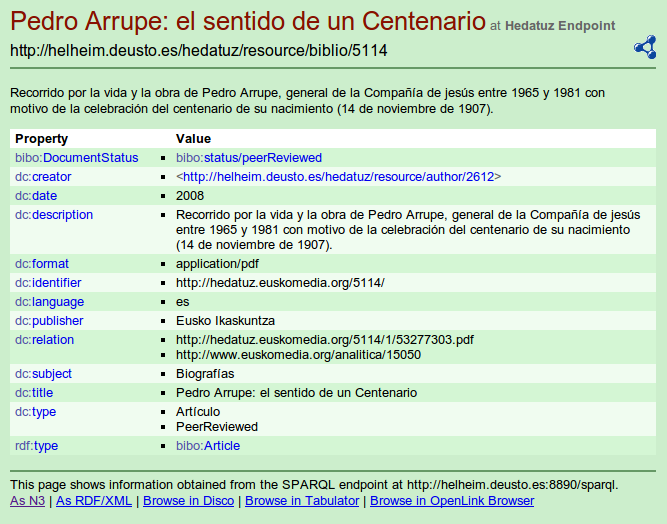
\includegraphics[width=0.92\textwidth]{img/ld_approach/pubby.png}
    \caption{Example of HTML visualization of a resource from Hedatuz dataset by Pubby.}
    \label{fig:pubby}
\end{figure}

D2R Server \cite{bizer2006d2r} allows the publication of relational databases as Linked Data. At first D2R requires the mapping of tables and columns from database to selected ontologies using D2RQ Mapping Language. Once this mapping is done, D2R offers a SPARQL endpoint to query data and a Pubby powered interface.

\begin{figure}
    \center
    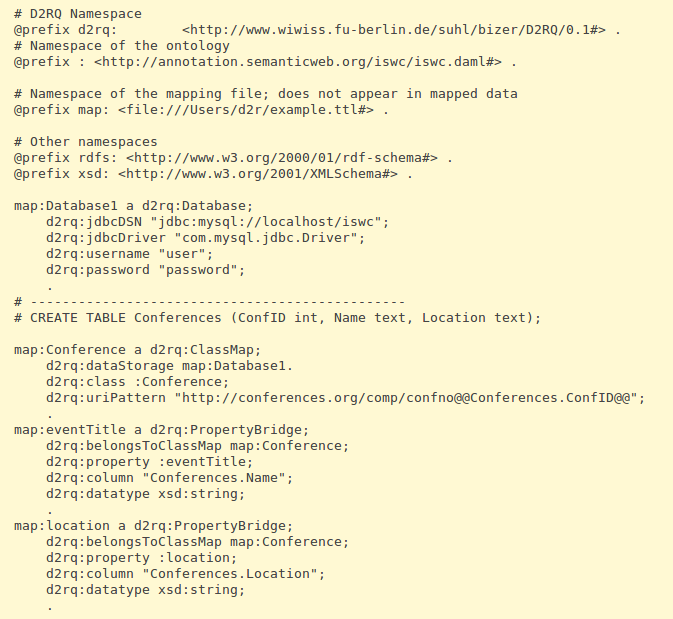
\includegraphics[width=0.98\textwidth]{img/ld_approach/d2rq.png}
    \caption{D2RQ mapping file. Example taken from http://d2rq.org/d2rq-language.}
    \label{fig:d2rq}
\end{figure}

In the process of publishing data from smart cities as Linked Data, new ontologies are going to be created to model the particularities of each city. The creators of these ontologies have to publish a suitable documentation, allowing the proper reuse of them. A tool for publishing ontologies and their documentation is Neologism\footnote{\url{http://neologism.deri.ie/}}. Neologism shows ontologies in a human-readable manner, representing class, subclass and property relationships through diagrams.

\subsection{Linkage}

Connecting existing data with other available resources is a major challenge for easing data integration. Due to its interlinked nature, Linked Data provides a perfect base to connect the data present in a given dataset.

The linkage stage starts a loop on the model after the publishing step, establishing relationships between existing data and external datasets, in order to provide links to new information stores.

Different frameworks have been developed to deal with class and properties matching. The basis of these frameworks is to provide data discovery features through links to external entities related to the items used in the analysis.

The \textit{Silk - Link Discovery Framework} \cite{volz2009silk} offers a flexible tool for discovering links between entities within different Web data sources. Silk makes use of \textit{Silk - Link Specification Language} (Silk-LSL), a declarative language which lets data publishers specify which RDF link types should be discovered providing two related datasets, and the conditions under data items must fulfill to be interlinked. As an example, a script in Silk-LSL can be written to match cities between \textit{DBpedia} ontology's \textit{City} or \textit{PopulatedPlace} classes, and \textit{GeoName}'s feature class \textit{gn:P}. As constraints, string similarity metrics can be used to match city names, and take into consideration cities' bounding boxes (i.e. the margins projected on a map) to check overlaps.

\begin{figure}
    \center
    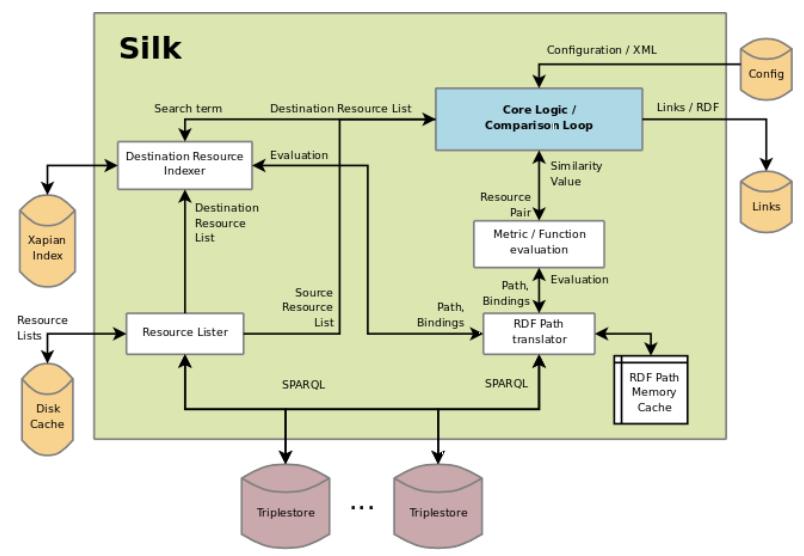
\includegraphics[width=0.75\textwidth]{img/ld_approach/silk.png}
    \caption{Silk framework architecture}
\end{figure}

With a similar approach \textit{LIMES} (LInk discovery framework for MEtric Spaces) \cite{ngomo2011limes} can be used for the discovery of links between Linked Data knowledge bases, focusing on a time-efficient approach especially when working with large-scale matching tasks. LIMES relies on \textit{triangle inequality} mathematical principles for distance calculations, which reduce the number of comparisons necessary to complete a mapping by several orders of magnitude. This approach helps detecting the pairs that will not fulfil the requirements in an early stage, thus avoiding spending time in more time-consuming processing.

\begin{figure}
    \center
    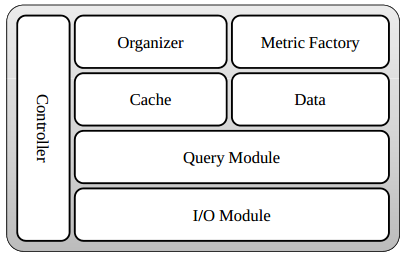
\includegraphics[width=0.5\textwidth]{img/ld_approach/limes.png}
    \caption{LIMES framework architecture}
\end{figure}

\subsection{Consume}
\label{subsec:consume}

At this stage, the focus is located on consuming data for business-logic processes, should they involve data mining algorithms, analytics, reasoning, etc.

Whereas complex processing algorithms can be used independently of the dataset format, Linked Open Data can greatly help at reasoning purposes. Linked Open Data describes entities using ontologies, semantic constraints and restriction rules (belonging, domain, range, etc.) which favor the inference of new information from the existing one. Thanks to those semantics present in Linked Data, algorithms are not fed with raw values (numbers, strings...), but with semantically meaningful information (height in cm, world countries, company names...), thus resulting in higher quality outputs and making algorithms more error aware (i.e., if a given algorithm is in charge of mapping the layout of a mountainous region, and founds the height of one of the mountains to be \textit{3.45}, it is possible to detect the conversion has failed at some point, as height datatype was expected to be given in \textit{meters}).

As seen in sections \ref{sensor_networks} and \ref{social_networks}, sensors and social networks are common data input resources, generating huge amounts of data streamed in real time. The work done in \cite{sequeda2009linked} comprises a set of best practices to publish and link stream data to be part of the Semantic Web.

However, when it comes to consume Linked Data streams, SPARQL can find its limits \cite{della2009s}. Stream-querying languages such as CQELS's\footnote{\url{https://code.google.com/p/cqels/}} language (an extension of the declarative SPARQL 1.1 language using the EBNF notation) can greatly help in the task. CQELS\cite{le2011native} (Continuous Query Evaluation over Linked Stream) is a native and adaptive query processor for unified query processing over Linked Stream Data and Linked Data developed at DERI Galway\footnote{\url{http://www.deri.ie/}}.

Initially, a query pattern is added to represent window operators on RDF Stream:

\begin{lstlisting}
GraphPatternNotTriples ::= GroupOrUnionGraphPattern |
OptionalGraphPattern | MinusGraphPattern | GraphGraphPattern |
*StreamGraphPattern* | ServiceGraphPattern | Filter | Bind
\end{lstlisting}

Assuming that each stream has an IRI as identification, the \textit{StreamGraphPattern} is defined as follows:

\begin{lstlisting}
StreamGraphPattern ::= 'STREAM' '['Window']' VarOrIRIref 
'{'TriplesTemplate'}'
Window ::= Rangle|Triple|'NOW'|'ALL'
Range ::= 'RANGE' Duration ('SLIDE' Duration |'TUMBLING')?
Triple ::= 'TRIPLES' INTEGER
Duration ::= (INTEGER 'd'|'h'|'m'|'s'|'ms'|'ns')+
\end{lstlisting}

An example query could be:

\begin{lstlisting}
PREFIX lv: <http://deri.org/floorplan/>
PREFIX dc: <http://purl.org/dc/elements/1.1/>
PREFIX foaf: <http://xmlns.com/foaf/0.1/>
PREFIX xsd: <http://www.w3.org/2001/XMLSchema#>

SELECT ?locName FROM NAMED <http://deri.org/floorplan/> 
WHERE {
	STREAM <http://deri.org/streams/rfid> [NOW]
	{?person lv:detectedAt ?loc}
	{?person foaf:name "AUTHORNAME"^^xsd:string }

	GRAPH <http://deri.org/floorplan/>
	{?loc lv:name ?locName}
}
\end{lstlisting}

Eventually, both batch and streamming results can be consumed through \textit{REST} services by web or mobile applications, or serve as input for more processing algorithms until they are finally presented to end-users.

\subsection{Visualize}

In order to make meaning from data, humans have developed a great ability to understand visual representations. The main objective of data visualization is to communicate information in a clean and effective way through graphical means. It's also suggested that visualization should also encourage users engagement and attention.

The \textit{"A picture is worth a thousand words"} saying reflects the power images and graphics have when expressing information, and can condense big datasets into a couple of representative, powerful images.

As Linked Data is based on subject-predicate-object triples, graphs are a natural way to represent triple stores, where subject and object nodes are inter-connected through predicate links. When further analysis is applied on triples, a diverse variety of representations can be chosen to show processed information: charts, infographics, flows, etc.\cite{khan2011data}

Browser-side visualization technologies such as d3.js\footnote{\url{http://d3js.org/}} (by Michael Bostock) and Raphaël\footnote{\url{http://raphaeljs.com/}} are JavaScript-based libraries to allow the visual representation of data on modern web browsers, allowing anybody with a minimum internet connection try to understand data patterns in a graphical form.

For developers not familiar with visualization techniques, some investigations are trying to enable the automatic generation of graphical representations of Linked Data query results. The \textit{LDVM} (Linked Data Visualization Model) \cite{brunetti2012linked} is proposed as a model to rapidly create visualizations of RDF data. \textit{LODVisualization}\footnote{\url{http://lodvisualization.appspot.com/}} is an implemented prototype which supports the LDVM.

Visualbox\footnote{\url{http://alangrafu.github.io/visualbox/}} is a simplified edition of LODSPeaKr\footnote{\url{http://lodspeakr.org/}} focused on allowing people create visualizations using Linked Data.

\begin{figure}
    \center
    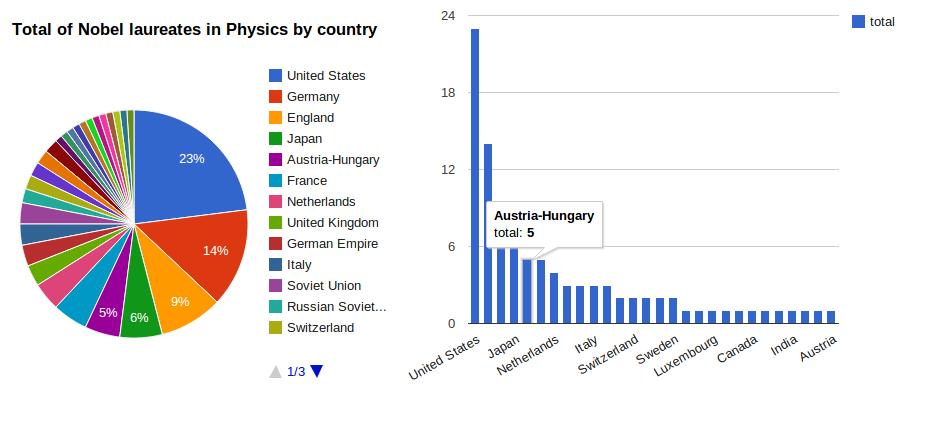
\includegraphics[width=\textwidth]{img/ld_approach/graph.png}
    \caption{Visualbox graph example (ownership: Alvaro Graves).}
\end{figure}

Independently of how visualizations are generated, they provide a perfect solution to present high-quality, refined data to end-users.

% Map4RDF
